\section{METHOD}
A VR twin is a fundamental interaction unit comprising a Real Interactive Object (RIO) in the physical world and its corresponding Virtual Interactive Object (VIO) in the virtual environment. The VIO provides visual feedback, while the RIO delivers haptic feedback. Crucially, VR twins enable users to interact through natural hand gestures without additional learning costs. Users perceive realistic haptic feedback during virtual interactions, mirroring the experience of manipulating real-world objects.

\subsection{Data Synchronization}
The VIO of VR twin synchronize the state (e.g., position, angle) of their corresponding RIO. Data communication between them is achieved through real-time sensing technology. Each of the three VR twins is equipped with specific sensors to capture the physical properties of the RIO, which is then filtered and transmitted to the VIO via Arduino for real-time updates.

\subsubsection{Sensing Solution}
\begin{enumerate}
  \item {\texttt{Puller}}: A combination of a tension sensor and an accelerometer is used. The tension sensor is installed at the connection point between the spring and the block to detect the pulling force applied by the user in real time. The accelerometer measures the block's acceleration, indirectly calculating its displacement and velocity. The tension sensor operates at a sampling frequency of 50 Hz, with a measurement range of 0 $N$ to 20 $N$ and an accuracy of $\pm$ 0.1 $N$. The accelerometer operates at 100 Hz, with a measurement range of $\pm$ 2 $m/s^2$ and a resolution of 0.01 $m/s^2$.

  \item {\texttt{Button}}: A thin-film pressure sensor is placed at the bottom of the spring. When the user presses the button, the spring's elasticity captures the applied pressure. The sensor operates at 100 Hz, with a measurement range of 0 $N$ to 10 $N$ and a resolution of 0.01 $N$.

  \item {\texttt{Knob}}: A high-precision angle sensor is integrated to detect the knob's rotation angle in real time. The angle sensor is installed at the center of the rotation axis, operating at 50 Hz with an accuracy of $\pm$ 0.5 degrees.
\end{enumerate}

\subsubsection{Data Communication}
Data communication is implemented using an Arduino UNO microcontroller and an HX711 module, enabling high-precision acquisition and transmission of analog sensor signals. The HX711 module is configured with a 128x gain to amplify and perform 24-bit analog-to-digital conversion on the signals from the thin-film pressure sensor and tension sensor, meeting high-precision measurement requirements.

The system adopts a distributed architecture, with three independent Arduino UNO microcontrollers connected to the thin-film pressure sensor, angle sensor, and tension sensor, respectively. Each microcontroller establishes a communication link with the computer via an independent USB serial port, enabling parallel data acquisition and transmission from multiple devices. On the computer side, multi-serial port communication technology is used to monitor multiple COM ports in real time, receiving data streams from different microcontrollers. The received data packets are parsed based on predefined device IDs and sensor type identifiers to extract valid measurements and store them in corresponding data structures.

\subsubsection{Data Processing}
During data acquisition, raw sensor data often contains noise due to environmental interference or sensor errors. The processing steps are as follows:

\begin{enumerate}
  \item {\texttt{Kalman Filtering}}: The Kalman filter algorithm is applied to the raw sensor data to predict and update the system state, reducing the impact of noise on data accuracy.

  \item {\texttt{Normalization}}: The processed data is normalized. At the start of the program, the initial sensor data is recorded as the lower input limit, corresponding to the RIO's initial state. The upper input limit is determined through 20 simulated input experiments, taking the maximum value. For the puller and button, the upper input limit is set to 800. For the knob, this step is omitted since it outputs angle data.

  \item {\texttt{Linear Interpolation}}: The normalized data is smoothed using linear interpolation. Let the data at time t be denoted as $x_{t}$. For the puller, if $x_{t}  > 0.05$, the block is considered pulled. If $\Delta x_{t} > 0.05$, the block is considered restored to its original position. For the button, if $x_{t}  > 0.05$, the button is considered pressed. If $x_{t} < 0.05$, the button is considered released. For the knob, its angle is synchronized in real time with $x_{t}$.
\end{enumerate}

\subsection{Virtual-Real Alignment}
Virtual-Real Alignment refers to the precise spaital and interactive matching and synchronization between the VIO and RIO of VR twins. The core objective is to ensure that users receive authentic and consistent visual and haptic feedback during interactions, thereby enhancing immersion and interactivity. Figure \ref{fig:teaser-right} illustrates the flowchart of virtual-real alignment.

\subsubsection{Spaital Alignment}
The RIOs of the three VR twins are fixed onto a portable plastic board, ensuring their relative positions remain constant. The plastic board serves as a reference benchmark, facilitating subsequent calibration and alignment operations. Based on the scale ratio between Unity and real-world space, the size and relative positions of the VIOs in the virtual scene are proportionally set to ensure their spatial positions fully correspond to those of the RIOs, as shown in Figure \ref{fig:spaital-alignment}.

\begin{figure}
  \centering
  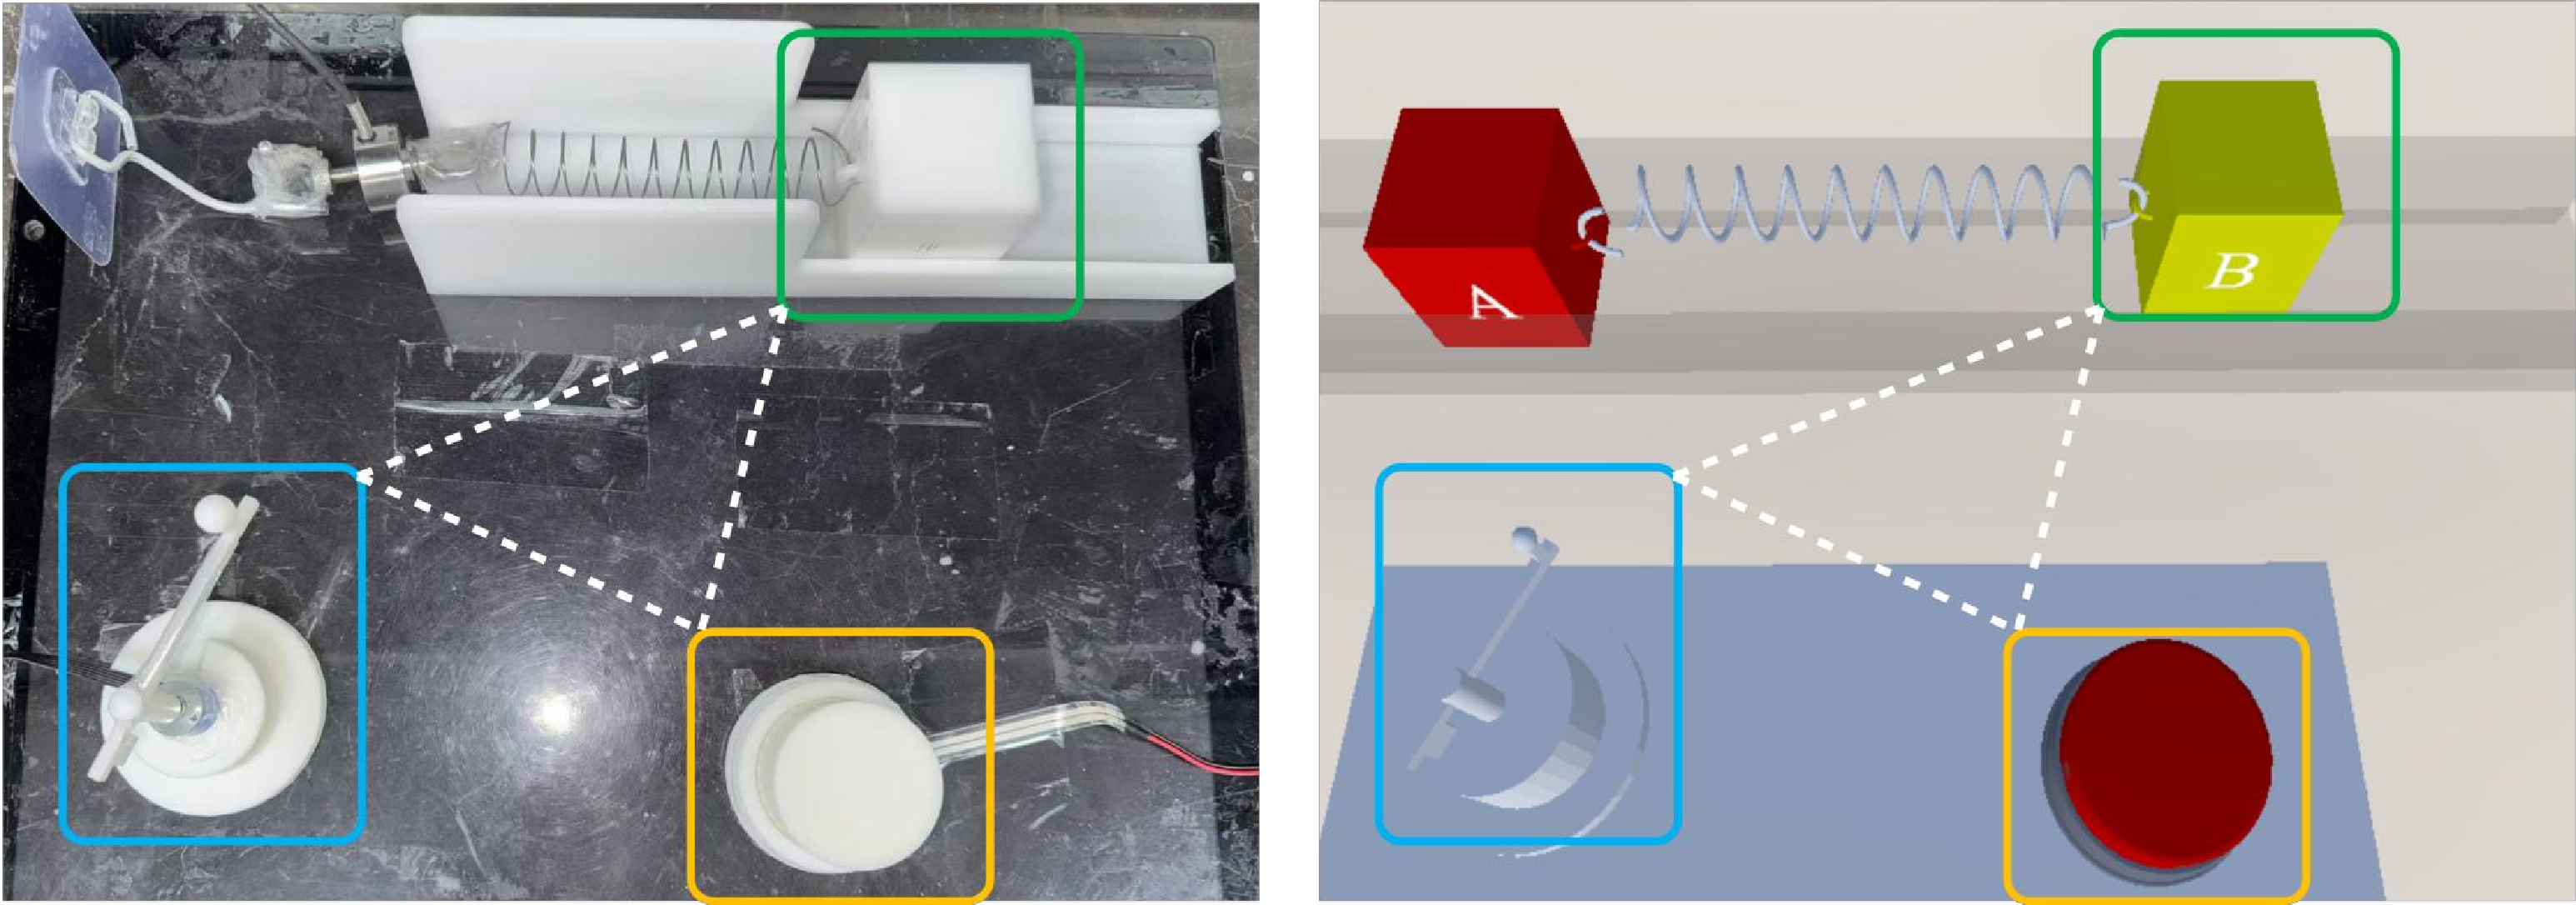
\includegraphics[width=\linewidth]{image/spaital-alignment.pdf}
  \caption{Spatial alignment of VIOs and RIOs.}
  \label{fig:spaital-alignment}
\end{figure}

During user interaction, let the processed data from the RIO at time $t$ be denoted as $x_{t}$. For the puller, the initial position of the VIO block is set as the origin (the spring's natural length), with the maximum pulling direction defined as the positive direction and the maximum pulling distance as $x_{max}$. The real-time horizontal coordinate of the block is calculated as $x_{t} \cdot x_{max}$. For the button, the initial height of the VIO switch is $h_{max}$, and the lowest height when pressed is $h_{min}$. The real-time height of the switch is $h_{max}-(h_{max}-h_{min}) \cdot x_{t}$. For the knob, the real-time angle of the VIO handle is synchronized with $x_{t}$.

\subsubsection{Interaction Calibration}
Although current gesture-tracking algorithms have made significant progress in stability and real-time performance, their recognition accuracy remains insufficient to support high-fidelity virtual-real alignment interactions. Specifically, positional and postural deviations caused by gesture-tracking errors can lead to penetration between the virtual hand and the VIO, where the virtual hand partially penetrates the object, causing visual distortion (Figure \ref{fig:gesture-tracking-deviations-b}). Traditional solutions often rely on physical collision detection to avoid penetration. However, this approach can lead to irregular motion of the object due to hand compression (Figure \ref{fig:gesture-tracking-deviations-c}), further degrading the user experience. To address this issue, our approach is divided into the following three steps.

\begin{figure}
  \begin{subfigure}{0.31\linewidth} % 子图 (a)
    \centering
    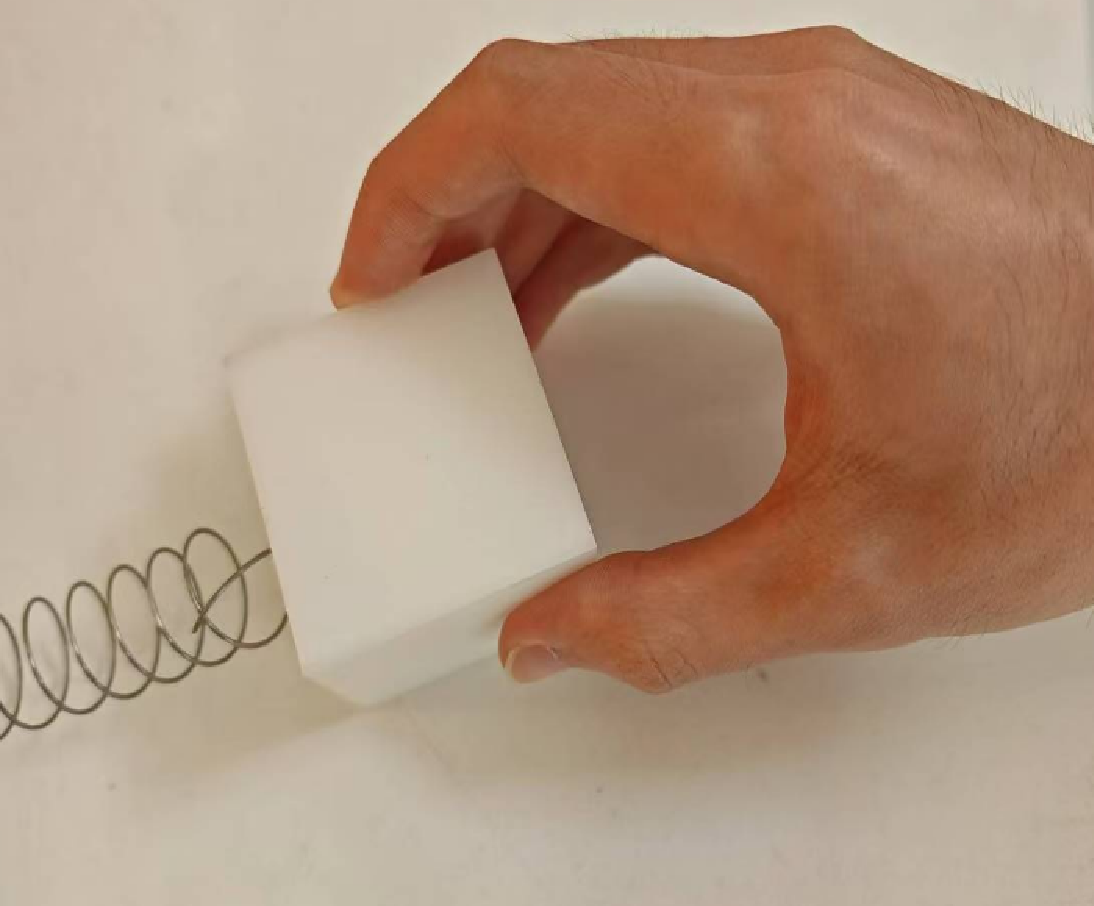
\includegraphics[width=\linewidth]{image/gesture-tracking-deviations-a.pdf}
    \caption{} % 子图标题 (a) 的内容
    \label{fig:gesture-tracking-deviations-a}
  \end{subfigure}
  \hfill % 水平填充间隔
  \begin{subfigure}{0.31\linewidth} % 子图 (b)
    \centering
    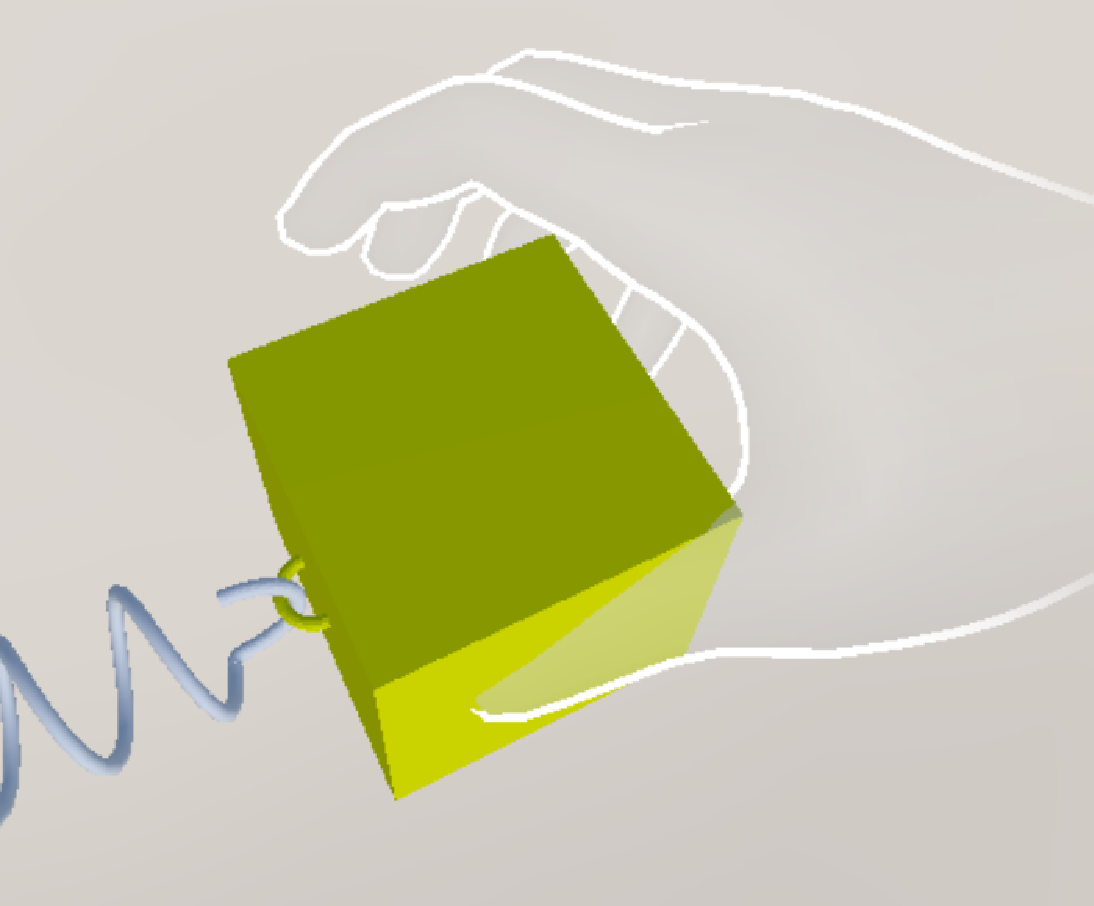
\includegraphics[width=\linewidth]{image/gesture-tracking-deviations-b.pdf}
    \caption{} % 子图标题 (b) 的内容
    \label{fig:gesture-tracking-deviations-b}
  \end{subfigure}
  \hfill % 水平填充间隔
  \begin{subfigure}{0.31\linewidth} % 子图 (c)
    \centering
    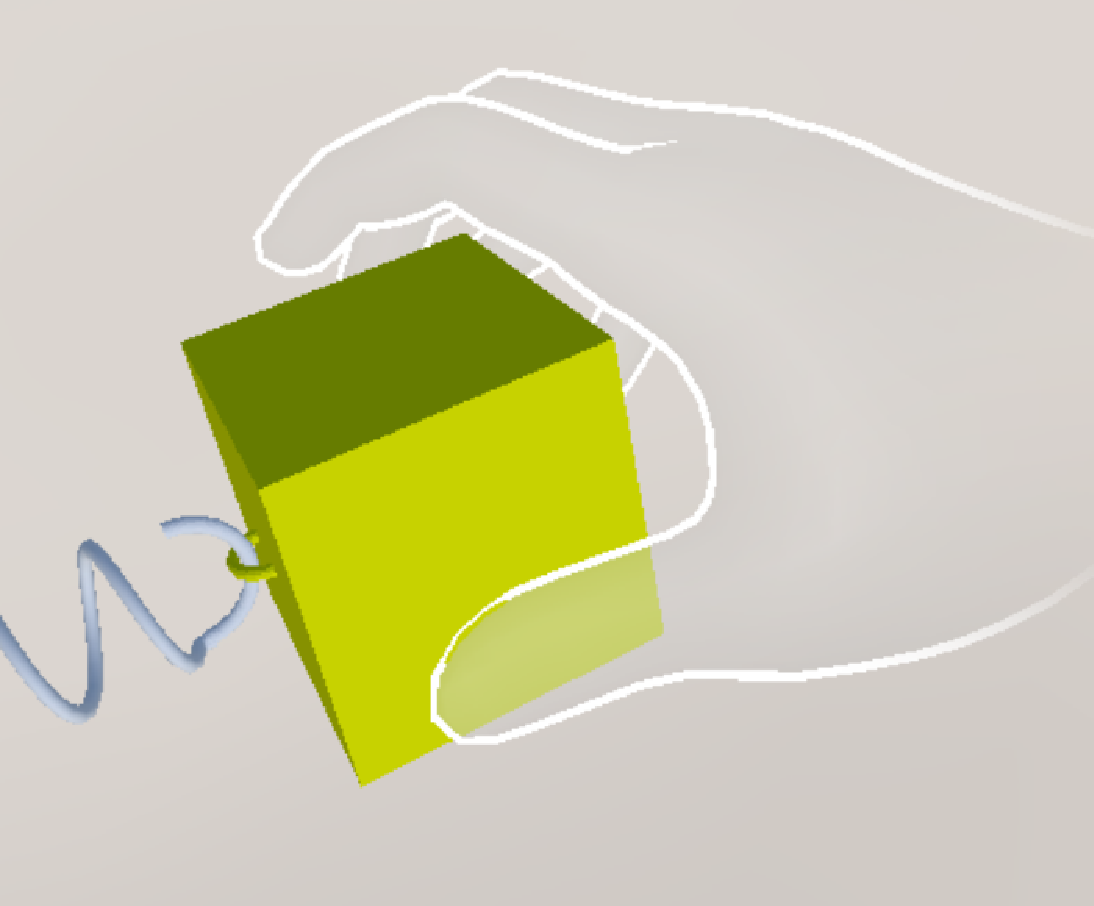
\includegraphics[width=\linewidth]{image/gesture-tracking-deviations-c.pdf}
    \caption{} % 子图标题 (c) 的内容
    \label{fig:gesture-tracking-deviations-c}
  \end{subfigure}
  \caption{Misalignment issue in gesture tracking. (\subref{fig:gesture-tracking-deviations-a}) Real interaction, (\subref{fig:gesture-tracking-deviations-b}) Virtual hand penetration, (\subref{fig:gesture-tracking-deviations-c}) Irregular object motion.}
  \label{fig:gesture-tracking-deviations}
\end{figure}

First, VIO's position, velocity, and angle are fully synchronized with RIO and remain unaffected by interactions in the virtual scene, meaning its mass property is infinity. This ensures that the virtual hand does not exert unintended physical effects on VIO during interaction.

Second, build parameterization of Gesture Characteristics, including finger joint positions, finger lengths, and finger bending angles, are parameterized. For the VIOs of three VR twins, predefined gestures that match the geometric features of the object surfaces are established. As shown in Figure \ref{fig:predefined-gestures}. For the puller, a semi-closed palm gesture with fingers encircling the object is defined. For the button, a flat palm gesture with fingers extended is defined. For the knob, a semi-closed palm gesture with fingers closed is defined.

\begin{figure}
  \begin{subfigure}{0.31\linewidth} % 子图 (a)
    \centering
    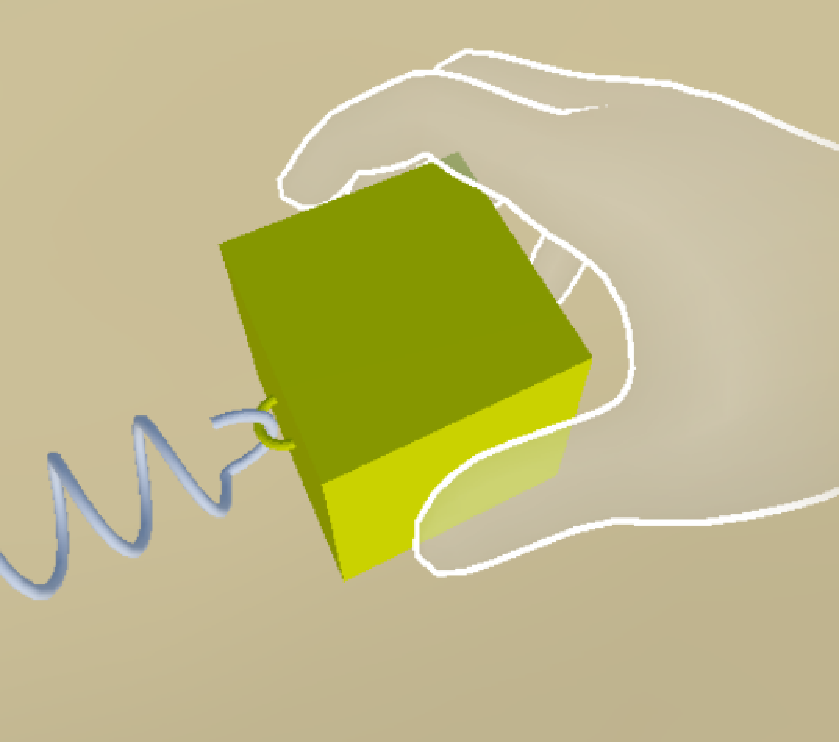
\includegraphics[width=\linewidth]{image/predefined-gesture-puller.pdf}
    \caption{} % 子图标题 (a) 的内容
    \label{fig:predefined-gestures-a}
  \end{subfigure}
  \hfill % 水平填充间隔
  \begin{subfigure}{0.31\linewidth} % 子图 (b)
    \centering
    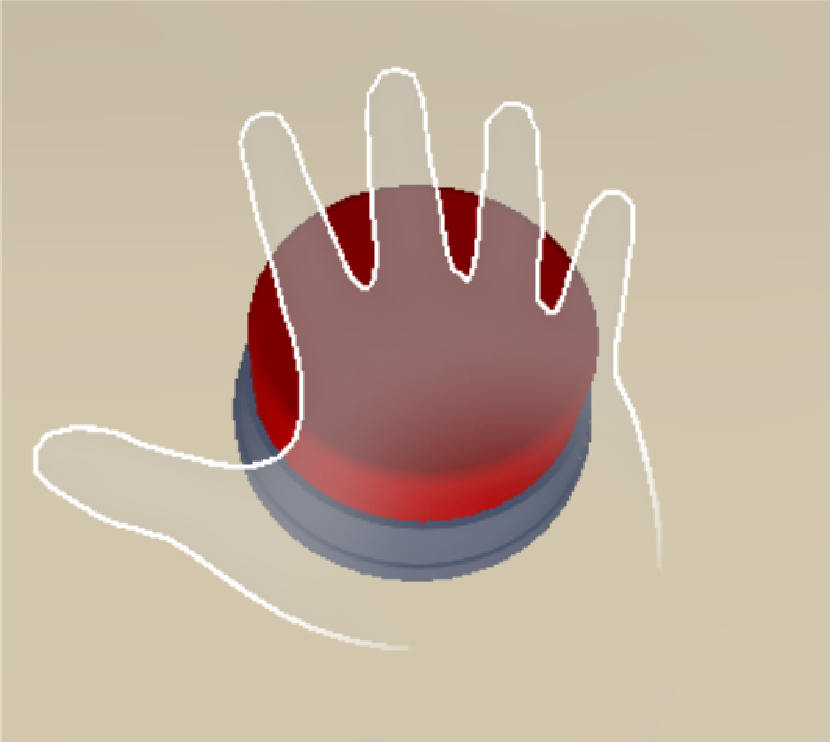
\includegraphics[width=\linewidth]{image/predefined-gesture-button.pdf}
    \caption{} % 子图标题 (b) 的内容
    \label{fig:predefined-gestures-b}
  \end{subfigure}
  \hfill % 水平填充间隔
  \begin{subfigure}{0.31\linewidth} % 子图 (c)
    \centering
    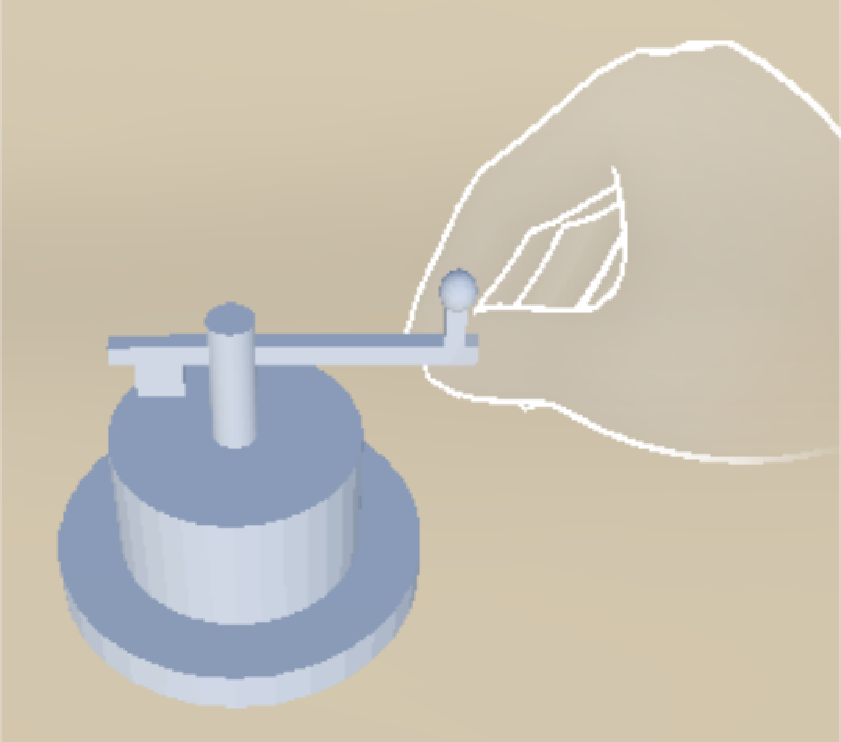
\includegraphics[width=\linewidth]{image/predefined-gesture-knob.pdf}
    \caption{} % 子图标题 (c) 的内容
    \label{fig:predefined-gestures-c}
  \end{subfigure}
  \caption{Predefined gestures for three VR twins. (\subref{fig:predefined-gestures-a}) Puller, (\subref{fig:predefined-gestures-b}) Button, (\subref{fig:predefined-gestures-c}) Knob.}
  \label{fig:predefined-gestures}
\end{figure}

Finally, interaction scheme is based on gesture prediction. A spherical bounding volume is constructed around the palm center as the detection region for interaction triggers, as shown in Figure \ref{fig:bounding-volume}. Additionally, a sphere tree model is built for hand joints (e.g., knuckles, palm center), as shown in Figure \ref{fig:sphere-tree-model}. During interaction, the system monitors gesture changes in real time and dynamically switches collision methods to ensure continuity and stability. When the VIO enters the spherical bounding volume's trigger region, the system begins predicting the user's gesture.

\begin{figure}
  \begin{subfigure}{0.48\linewidth} % 子图 (a)
    \centering
    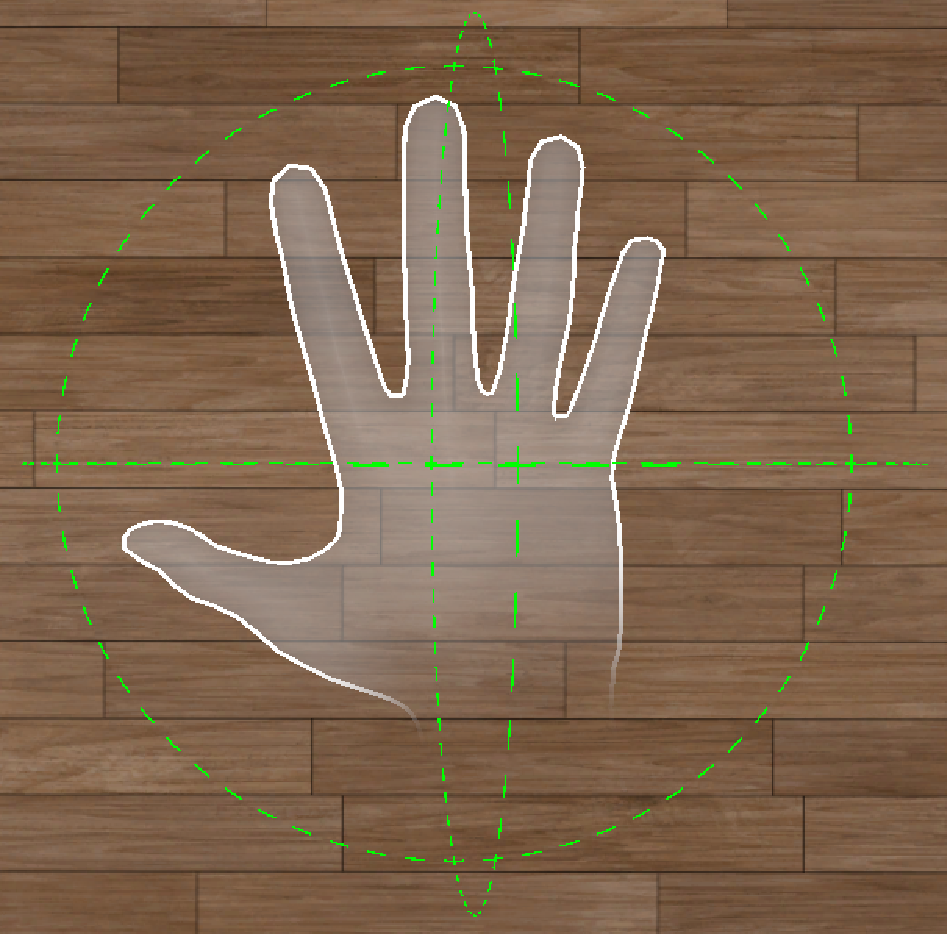
\includegraphics[width=\linewidth]{image/bounding-volume.pdf}
    \caption{} % 子图标题 (a) 的内容
    \label{fig:bounding-volume}
  \end{subfigure}
  \hfill % 水平填充间隔
  \begin{subfigure}{0.48\linewidth} % 子图 (b)
    \centering
    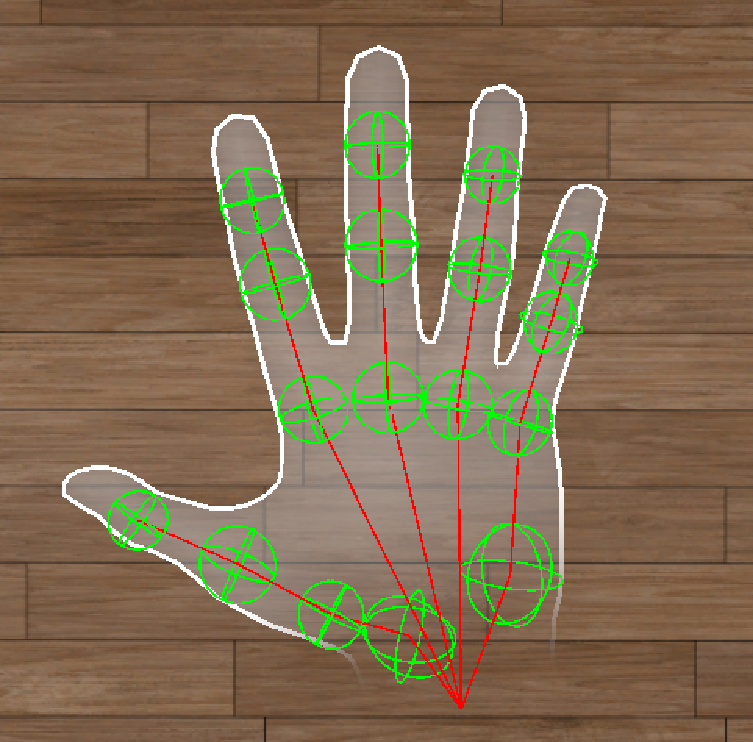
\includegraphics[width=\linewidth]{image/sphere-tree-model.pdf}
    \caption{} % 子图标题 (b) 的内容
    \label{fig:sphere-tree-model}
  \end{subfigure}
  \caption{Bounding volume and sphere tree model for the virtual hand. (\subref{fig:bounding-volume}) Spherical bounding volume, (\subref{fig:sphere-tree-model}) Sphere tree model.}
  \label{fig:bounding-volume-and-sphere-tree-model}
\end{figure}

\begin{enumerate}
  \item {\texttt{Interacting}}: When the user's gesture matches the predefined interaction gesture and contacts the VIO, the system determines that the user is performing an interaction operation. As shown in Figure \ref{fig:interacting-scheme}, the blue squares and red connecting lines represent the gesture-tracking results, with some joints penetrating the object due to errors. At this point, an interpolation method smoothly transitions the virtual hand from its current posture to the predefined interaction gesture (outlined in white), and the sphere tree model's physical collision is disabled to prevent penetration.

  \item {\texttt{Non-Interacting}}: In other cases, where the user is not interacting with the VIO, the sphere tree model's physical collision prevents the virtual hand from penetrating the VIO. As shown in Figure \ref{fig:non-interacting-scheme}, the user places their hand flat above the object, and the collision bodies of the hand joints constrain the virtual hand's penetration. Since the object has infinite mass, irregular motion does not occur.
\end{enumerate}

\begin{figure}
  \begin{subfigure}{0.48\linewidth} % 子图 (a)
    \centering
    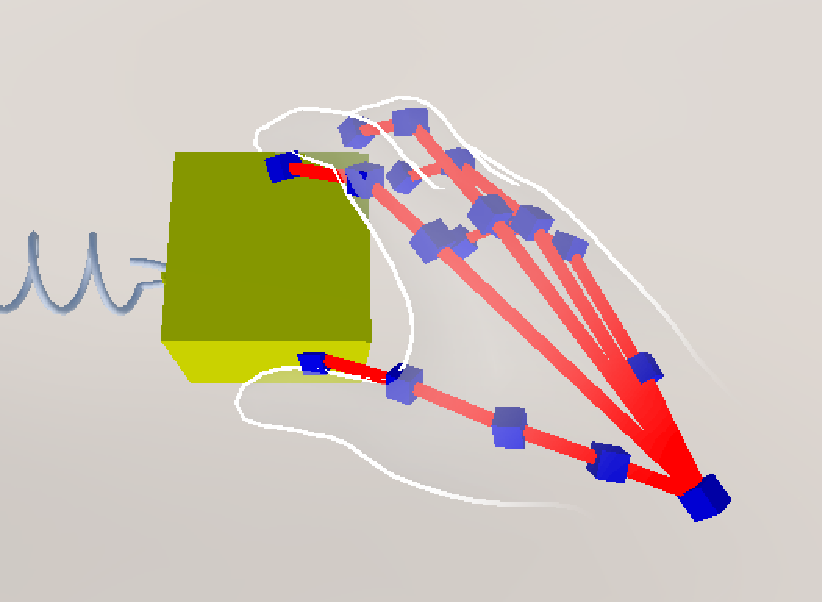
\includegraphics[width=\linewidth]{image/interacting-scheme.pdf}
    \caption{} % 子图标题 (a) 的内容
    \label{fig:interacting-scheme}
  \end{subfigure}
  \hfill % 水平填充间隔
  \begin{subfigure}{0.48\linewidth} % 子图 (b)
    \centering
    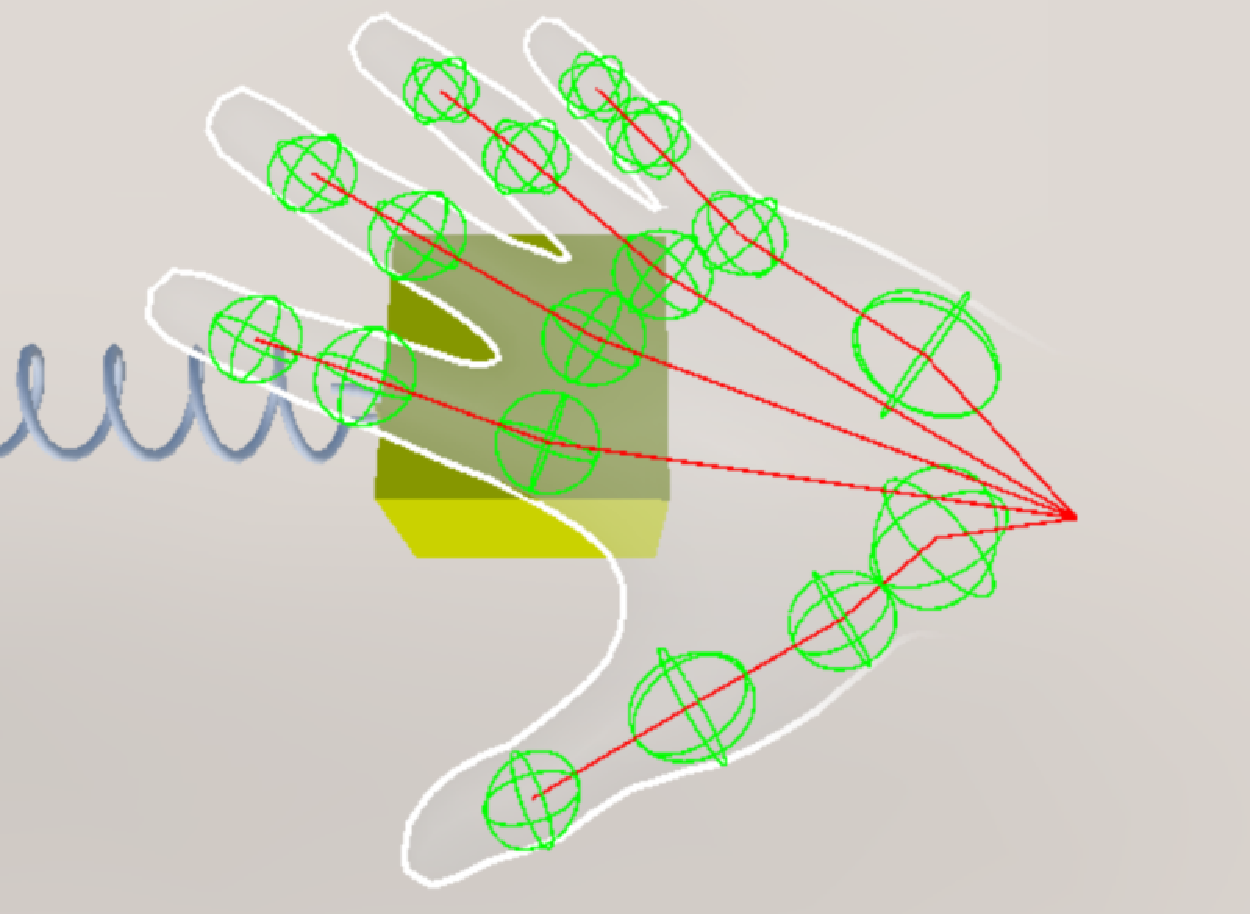
\includegraphics[width=\linewidth]{image/non-interacting-scheme.pdf}
    \caption{} % 子图标题 (b) 的内容
    \label{fig:non-interacting-scheme}
  \end{subfigure}
  \caption{Interaction scheme based on gesture prediction. (\subref{fig:interacting-scheme}) Interacting, (\subref{fig:non-interacting-scheme}) Non-interacting.}
  \label{fig:interaction-scheme}
\end{figure}